\section{Projeto Estrutural}
O projeto estrutural tem como fun\c{c}\~{a}o suportar todos os componentes do sistema; suportar os esfor\c{c}os impostos pela pr\'{o}pria carga dos componentes al\'{e}m de cargas externas previstas na rotina de usabilidade do sistema e eventuais.

A proposta real para carga \'{e} de 300kg de ra\c{c}\~{a}o, por\'{e}m foi constru\'{o} parcialmente em escala real e parcialmente em escala de 1:6, devido a dificuldades de locomo\c{c}\~{a}o e esfor\c{o} f\'{i}sico para transportar a carga de 300kg, fator que n\~{a}o teria influ\^{e}ncia no teste de determinados componentes do sistema. \\

A divis\~{a}o estrutural dos componentes \'{e} disposta da seguinte forma:

%	\item[estr] - \textbf{Estrutura Flutuadora}
%	\item[flut] - \textbf{Estrutura de Sustenta\c{c}\~{a}o}
%	\item[arm] -\textbf{ Armazenadores}
  \subitem Armazenador Principal
  \subitem Armazenador de Dosagem


\subsection{Armazenador Principal}
O armazenador principal comportar\'{a} toda a carga de ra\c{c}\~{a}o calculada para o per\'{i}odo estipulado pelo cliente, caso 300kg, o que ser\'{a} suficiente para alimentar os peixes do tanque rede por 4 dias, per\'{i}odo em que h\'{a} maior taxa de mortalidade e perda de produtividade no criat\'{o}rio.

Projetado e constru\'{i}do com cantoneiras e chapas de alum\'{i}nio devido \`{a} resist\^{e}ncia ao ambiente de atua\c{c}\~{a}o do sistema. Seu baixo peso acima do n\'{i}vel da \'{a}gua foi um dos principais motivos para escolha do material, pois evita que o centro de gravidade da massa suportada pela estrutura sustentadora fique elevado em rela\c{c}\~{a}o ao n\'{i}vel da \'{a}gua, j\'{a} que a eleva\c{c}\~{a}o deste prejudicaria a estabilidade do sistema.

A fixa\c{c}\~{a}o das contoneiras foi feita atrav\'{e}s de solda. Embora a solda de alum\'{i}nio estivesse dispon\'{i}vel, as chapas foram rebitadas, devida a sua baixa espessura, o que dificulta bastante o processo de soldagem.

Segundo a simula\c{c}\~{a}o, a integridade estrutural do armazenador ser\'{a} totalmente preservada, com fator de seguran\c{c}a  em torno de 20. O elevado fator de seguran\c{c}a n\~{a}o se deve a superdimensionamento, e sim devido ao fato do material escolhido de acordo com acessibilidade e manufaturabilidade possuir elevada resist\^{e}ncia estrutural para a devida aplica\c{c}\~{a}o.

\begin{figure}[h]
  \centering
  \includegraphics[width=4in]{figuras/Armazenador_Tensao}
  \caption{Tens\~{a}o Armazenador Principal - "Ponto Cr\'{i}tico}
\end{figure}

\begin{figure}[h]
\centering
\includegraphics[width=4in]{figuras/armazenadorPrincipal}
\caption{Armazenador Principal}
\end{figure}

\subsection{Armazenador de Dosagem}
O armazenador de dosagem ser\'{a} respons\'{a}vel por armazenar a dose correta para cada trato e conter\'{a} ra\c{c}\~{a}o durante a pesagem da dose para que esta possa ser despejada nos tanques. Segundo informa\c{c}\~{o}es do usu\'{a}rio, a capacidade de 10kg por trato \'{e} o suficiente.\textit{Este foi constru\'{i}da em escala para o prot\'{o}tipo, assim como combinado com os professores da disciplina e explicado no inicio do trabalho.} \\


Portanto, o dosador foi projetado e constru\'{i}do de forma que o fundo tivesse a angula\c{c}\~{a}o necess\'{a}ria para o escoamento da ra\c{c}\~{a} sem que haja a necessidade de um atuador para despeja-la. Essa inclina\c{c}\~{a}o foi determinada por meio de testes em um dispositivo constru\'{i}do pela pr\'{o}pria equipe com os materiais utilizados no sistema real. \\



  \begin{figure}[h]
    \centering
    \includegraphics[width=4in]{figuras/sistema_lago}
    \caption{Sistema no lago}
  \end{figure}

E o ângulo de caída para as rações desde a menor gramatura até a maior foi de 15\textdegree < $\theta$ < 20\textdegree.

% E o \^{a}ngulo de ca\'{i}da para as ra\c{c}\~{o}es desde a menor gramatura até a maior foi 15\textdegree < \text{\theta} < 20\textdegree.
% s

A escolha do material, chapas de alum\'{i}nio, se deu pelos mesmos fatores do armazenador principal, j\'{a} que o dosador tamb'{e}m est\'{a} acima da linha da \'{a}gua e tem resist\^{e}ncia aos esfor\c{c}os nele aplicados, obtendo fator de seguran\c{c}a em torno de 4.5.\textit{Este foi constru\'{i}da em escala para o prot\'{o}tipo, assim como combinado com os professores da disciplina e explicado no inicio do trabalho.}\\


\begin{figure}[h]
  \centering
  \includegraphics[width=4in]{figuras/Dosador_Tensao}
  \caption{Tens\~{a}o Dosador}
\end{figure}


\subsection{Estrutura de Sustenta\c{c}\~{a}o}

A estrutura de sustenta\c{c}\~{a}o \'{e} respons\'{a}vel por fazer a conex\~{a}o entre todos esses componentes e suportar os esfor\c{c}os nela aplicados. Esta foi constru\'{i}da em escala para o prot\'{o}tipo, assim como combinado com os professores da disciplina e explicado no inicio do trabalho

As cantoneiras de alum\'{i}nio foram escolhidas como material devido aos mesmos fatores que implicaram na escolha do material do armazenador principal e dosador.

A simula\c{c}\~{a}o estrutural realizada demonstrou que h\'{a} capacidade de sustentar todos os outros componentes com fator de seguran\c{c}a em torno de 10.


\begin{figure}
\centering
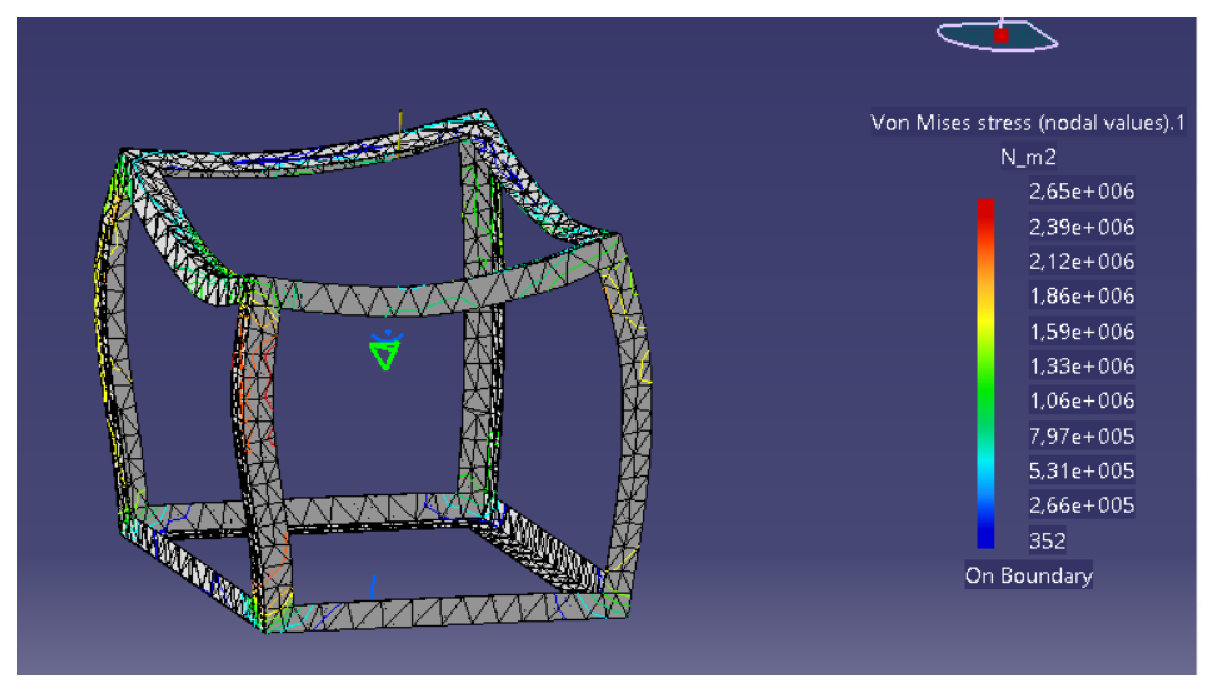
\includegraphics[width=4in]{figuras/Sustentacao_tensao}
\caption{Tens\~{a}o Estrutura de Sustenta\c{c}\~{a}}
\end{figure}

\subsection{Estrutura Flutuadora}

A estrutura flutuadora tem a responsabilidade de sustentar acima do n\'{i}vel da \'{a}gua todos os componentes para que se possibilite o correto funcionamento do sistema.

Diferente da escolha do material do restante da estrutura, foi escolhido tubos de se\c{c}\~{a}o quadrada de a\c{c}o devido principalmente a dois fatores que atrelados predominaram em rela\c{a}o aos outros. Para a estabilidade, a \'{a}rea e massa da estrutura submersa tem forte influ\^{e}ncia na estabilidade. Portanto foi escolhido o a\c{c}o como material devido ao seu elevado peso e baixo custo em rela\c{c}\~{a}o ao alum\'{i}nio.

Para proteger esta estrutura que ficar\'{a} submersa da oxida\c{c}\~{a} esta ser\'{a} revestida com batida de pedra, o mesmo material utilizado para proteger chassis e partes inferiores de ve\'{i}culos.

Assim como os outros componentes, a simula\c{c}\~{a} demonstrou que a estrutura projetada pode suportar os esfor\c{c}os aplicados com alto fator de seguran\c{c}a e baix\'{i}ssima deforma\c{c}\~{a}o. \textit{Esta foi constru\'{i}da em tamanho real para que a estabilidade pudesse ser testada de fato, com valores de aplica\c{c}\~{a}o.}\\

\begin{figure}
  \centering
  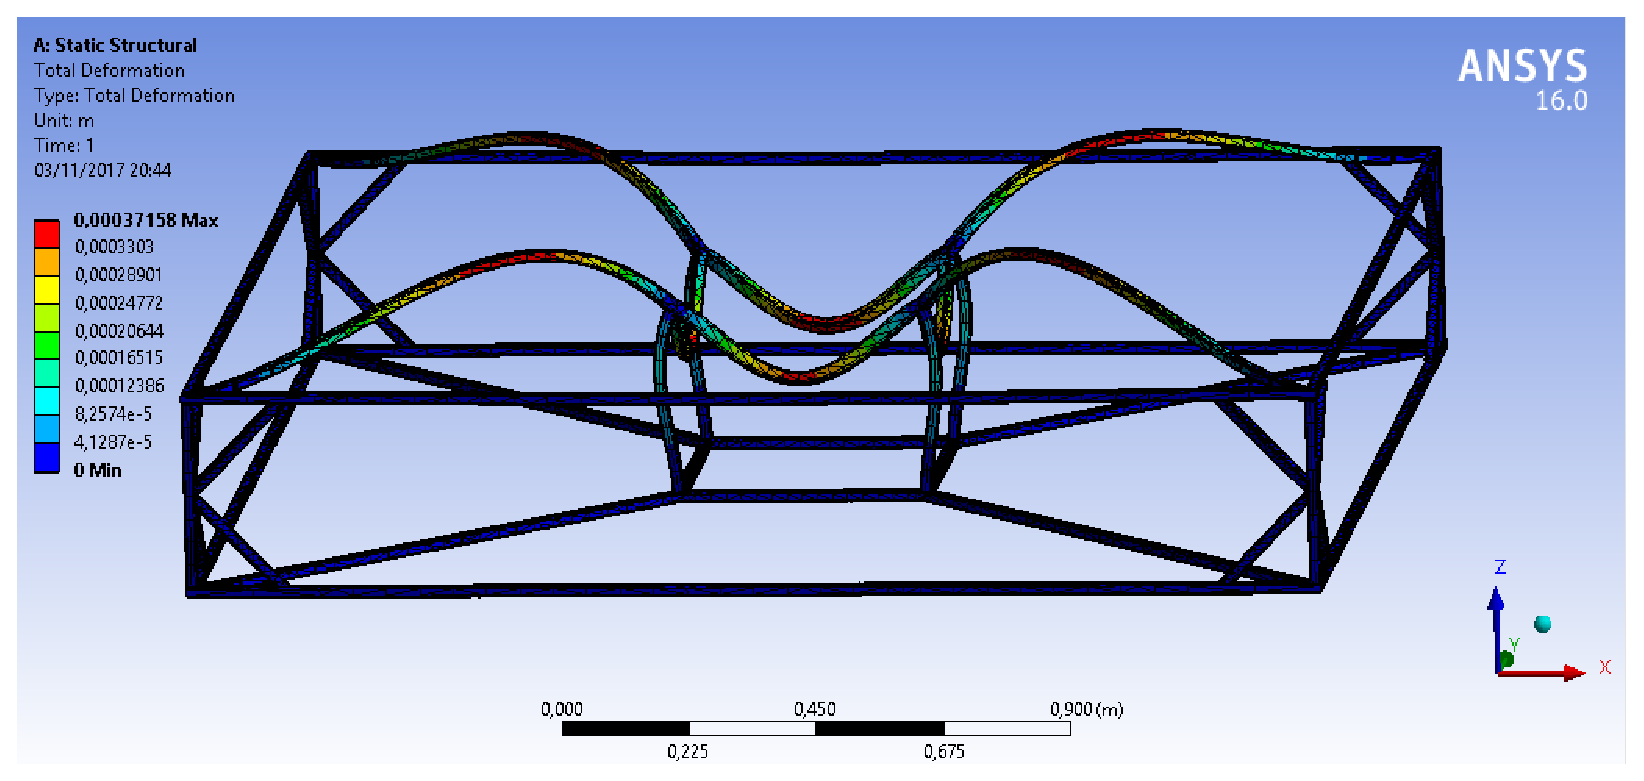
\includegraphics[width=4in]{figuras/Deformacao_EstruturaSust}
  \caption{Tens\~{a}o Estrutura Flutuadora}
\end{figure}
